\documentclass[10pt]{article}
\usepackage[T1]{fontenc}
\usepackage{amssymb}
\usepackage{amsmath}
\usepackage{graphicx}
\usepackage{algpseudocode}
\usepackage{algorithm}



\usepackage{tikz}
\usetikzlibrary{arrows}
\usepackage{subfigure}
\usepackage{stackrel}
\usepackage{blindtext}
\usepackage{scrextend}
\addtokomafont{labelinglabel}{\sffamily}

\usepackage{biblatex}
\addbibresource{library.bib}

\oddsidemargin=0.15in
\evensidemargin=0.15in
\topmargin=-.5in
\textheight=9in
\textwidth=6.25in

\usepackage[colorlinks=true,breaklinks,pdfpagemode=none,linkcolor=blue,citecolor=blue]{hyperref}
\usepackage{enumerate}

%\usepackage{enumitem}
%\setlist{itemsep=0mm}



%\usepackage[usenames,dvipsnames]{pstricks}
%\usepackage{epsfig}
\usepackage{amsmath,amsfonts,amssymb,bm}
%\usepackage{pst-grad} % For gradients
%\usepackage{pst-plot} % For axes


%% Environment definitions (add your own here)

\newtheorem{theorem}{Theorem}
\newtheorem{corollary}[theorem]{Corollary}
\newtheorem{lemma}[theorem]{Lemma}
\newtheorem{observation}[theorem]{Observation}
\newtheorem{proposition}[theorem]{Proposition}
\newtheorem{definition}[theorem]{Definition}
\newtheorem{claim}[theorem]{Claim}
\newtheorem{fact}[theorem]{Fact}

\newenvironment{proof}{\noindent{\bf Proof}\hspace*{1em}}{\qed\bigskip}

%% New commands (add your own here)

\newcommand{\eps}{\varepsilon}
\newcommand{\bbR}{\mathbb{R}}
\newcommand{\hv}{\hat{v}}
\newcommand{\hL}{\hat{L}}
\newcommand{\hlambda}{\hat{\lambda}}
\newcommand{\homega}{\hat{\omega}}
\newcommand{\hp}{\hat{p}}
\newcommand{\hW}{\hat{W}}
\newcommand{\cK}{\mathcal{K}}
\newcommand{\qed}{\rule{7pt}{7pt}}
\newcommand{\cF}{\mathcal{F}}



\begin{document}

   \noindent
   \begin{center}

   \hrulefill
   
   \vspace{5pt}
   
   \makebox[\textwidth]{ {\bf Energy Systems Analysis} \hfill  A.D. Smith 2019}
   \vspace{0pt}
   
   {\Large \hfill Introduction: Analysis \& Modeling of Energy Systems}
   \vspace{5pt}
   
  
   \hrulefill
   \end{center}

{\color{darkgray}{\center{ \small{      ``The best thing to do is start simply and then build in complexity. Do the dumbest thing you can think of first.''
\\%[3pt]
\rightline{{\rm --- O'Neil and Schutt \cite{Schutt2013-kj}}}}}}}

\section{Analyzing energy systems}
In an excellent book called \textit{How to Solve It} \cite{polya}, G. Polya presents a very general approach that can be applied to the analysis of energy systems. [My comments in brackets]

\begin{quote}
\begin{labeling}{longest}
\item [\textbf{First}] You have to \textit{understand} the problem. \cite{polya} [No small feat for complex energy systems!]
\item [\textbf{Second}] Find the connection between the data and the unknown \ldots You shoud obtain eventually a \textit{plan} of the solution. \cite{polya} [If that connection isn't there, it's time to back up to your data search or collection process.]
\item [\textbf{Third}] \textit{Carry out} your plan. \cite{polya} [And \textit{evaluate} your progress as you go.]
\item [\textbf{Fourth}] \textit{Examine} the solution obtained. \ldots Can you \textit{check the result}?  \cite{polya} [Verification/validation often require critical thinking and creativity.]

\end{labeling}
\end{quote}

\section{Working energy system problems}

Many of the same techniques that are good for tackling thermal-fluid science or problems will be effective at energy systems problems.
{\fontfamily{cmss}\selectfont
\begin{enumerate}
    \item Identify the system of interest.
    \item Define the question you want to investigate.
    \item Determine what you could measure or evaluate to address your question.
    \item Determine the level of detail to start with according to the temporal and spatial dimensions of interest.
    \item Decide what to measure or evaluate, starting with the simplest option(s).
    \item Apply relevant methods for your model or experiment.
    \item Assess what you've learned from the model or experiment.
    \item Revisit the question you defined, considering whether you want to change it or investigate further.
    \item Reassess the level of detail and methods, considering whether you've adequately answered the question.
    \item Explain your results, documenting your methods and the analytical process itself.
\end{enumerate}
}

The fundamental equations guiding the behavior of energy consuming or energy conversion devices often boil down to the first and second laws of thermodynamics. But the fundamental concepts of systems problems are not quite so clear--often the behavior of a number of things working together is not an obvious combination of anything.

%remove this quote here as it is used in opt. lecture (42). write my interpretation of what schutt means.
I like the quote above (``do the dumbest thing'') because they're poking a little fun at us, and engineers or scientists often seem to get ahead of ourselves. I find that often when students say, ``I don't know what to do'' they actually do have ideas, it's just they're not convinced they're right.

Starting with something that seems dead simple or obvious may give you a concrete starting point for your analysis or optimization, or may leave you with a new understanding that you couldn't have gained without actually trying something yourself. This holds true for building things, experimentation, analytical work and model creation as well. %great for engineers



\section{Creating models of energy systems}
In his classic modeling text \textit{Mathematical Modelling Techniques}, Rutherford Aris defines a \textit{mathematical model} as ``any complete and consistent set of mathematical equations which is thought to correspond to some other entity.'' \cite{aris} Like Aris, we will abbreviate `mathematical model' to simply `model' and in this course, we will often be referring to a model that is implemented computationally, where the model is some combination of code and data structures.

\begin{quote}
The formulation of the equations of a model is usually a matter of expressing the physical laws or conservation principles in appropriate symbols. \cite{aris}    
\end{quote}


In creating (or `formulating') a model, we will be concerned with the behavior over time of systems based on the equations governing energy and mass conservation and, to a lesser extent, entropy generation, as these laws describe the conversion of energy and the performance of engineered systems that convert or store energy. 

\section{Integrated analysis method}

{\fontfamily{cmss}\selectfont
\begin{enumerate}[(i)]
    \item Identify the system of interest.
    \item Define the question you want to investigate.
    \item Determine what you could measure or evaluate to address your question.
    \item Determine the level of detail to start with according to the temporal and spatial dimensions of interest.
    \item Decide what to measure or evaluate, starting with the simplest option(s).
    \item Apply relevant methods for your model or experiment.
    \item Assess what you've learned from the model or experiment.
    \item Reassess the question you defined, considering whether you want to change it or investigate further.
    \item Reassess the level of detail and methods, considering whether you've adequately answered the question.
    \item Explain your results, documenting your methods and the analytic process itself.
\end{enumerate}
}

See Figure \ref{IAM}, where the iterative nature of the process is illustrated graphically.


\medskip
            \begin{figure}[h]
            \centering
            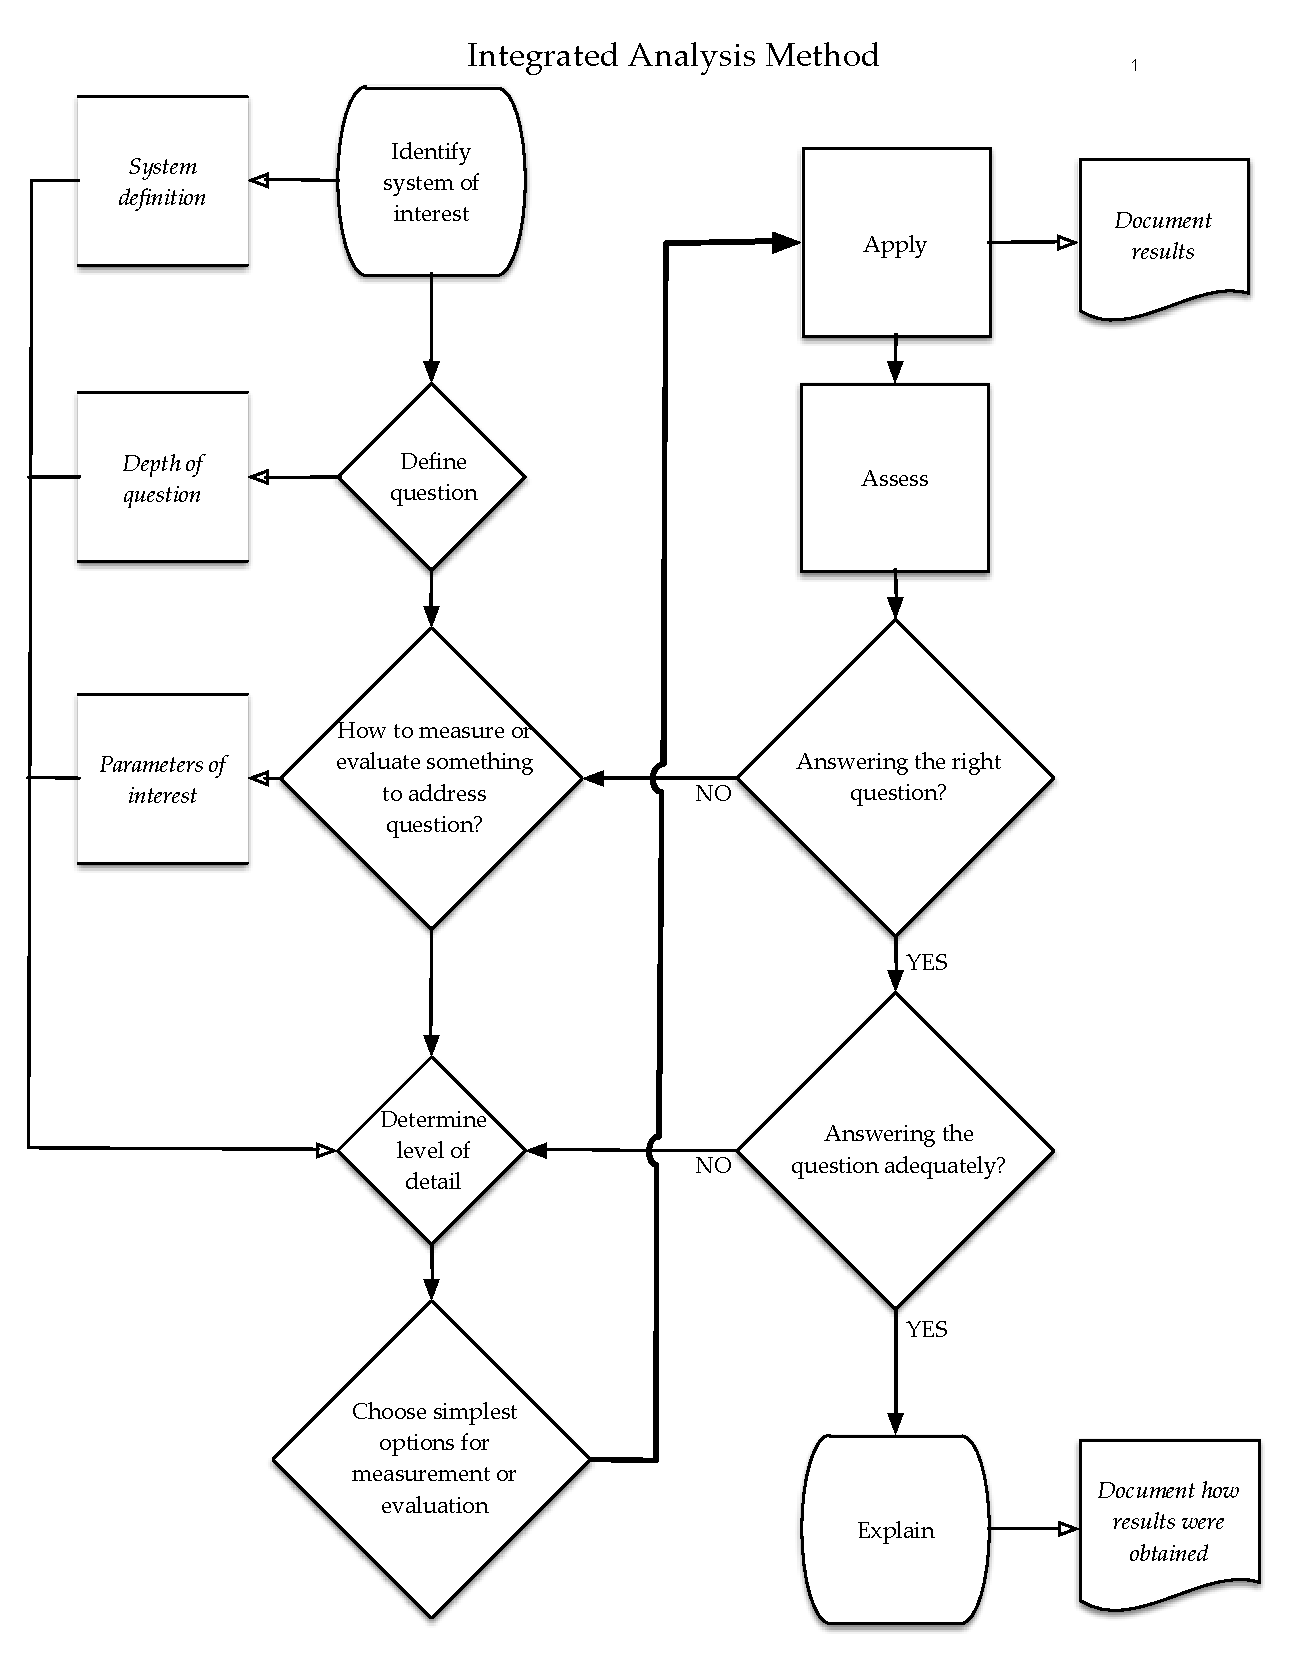
\includegraphics[width=6in]{extras00/IAMoverview.pdf}
            \caption{Integrated Analysis Method overview}
            \label{IAM}
            \end{figure}
\bigskip

\section{Important Terms}

\begin{labeling}{longest}
\item [\textbf{energy}] the currency for work, which is a force being moved through a distance, or equivalent quantity. [Units will be force $\times$ distance (also electric charge $\times$ electric potential) or power $\times$ time.]
\item [\textbf{power}] rate of delivering energy. [Units will be energy $\div$ time.]\\
\item [\textbf{validation}] Do my results line up with observed data?
\item [\textbf{verification}] Did I actually do what I think I did?
\end{labeling}

% Add section on common energy units

\bigskip

\noindent
\texttt{\footnotesize RESTRICTED PUBLIC LICENSE --- READ BEFORE SHARING. This is a draft version made available by Amanda D. Smith under a Creative Commons Attribution-NonCommercial-ShareAlike license. 
\href{https://creativecommons.org/licenses/by-nc-sa/4.0/}{CC BY-NC-SA 4.0}}

% references
\printbibliography

\end{document}